\documentclass{article}
%\usepackage[utf8]{inputenc}
\usepackage{graphicx}
\usepackage[T1]{fontenc}
\usepackage[section]{placeins}
\usepackage[a4paper, total={5.5in, 8in}]{geometry}
\usepackage{float}
\usepackage{indentfirst}
\title{HD Spectroscopy and the Hydogen Isotope Shift}
\author{Baskar Dutt and Jack Roten}
\date{Thursday January 31, 2019}

\begin{document}
\maketitle

\section{Abstract}

In this lab we observe the Balmer series of Deuterium and Hydrogen in order to demonstrate the relationship between the mass of the nucleus and the energy spectrum. This is done by using a spectrometer to separate the emitted wavelengths of the sample, which is then captured by the photomultiplier that sends a signal of the amplitude to the computer data collector software. We find our results to be close to theoretical prediction with and error o at most 2.9\%.



\section{Introduction}

Spectroscopy is the study of interaction between matter and electromagnetic radiation.  The notion of discrete energy levels of electrons in atoms, ions, or molecules was first introduced by Niels Bohr and further understood by Rutherford-Bohr Model before the formulation of wave equations and quantum mechanics.  When transitions from a higher energy state to a lower energy state occurs, energy is released in a photon characterized by a wavelength.  The Rydberg equation specifies this relationship and is given by the following: $\frac{1}{\lambda} = Ry\frac{M}{m_e+M}(\frac{1}{n_f^2}-\frac{1}{n_i^2})$. In this experiment we examine the relationship between the reduced mass and energy transitions by experimentally observing the shift in energy released from a state $n_f$ to $n_i$  of $H_2$ and $D_2$ with $n_f = 2$. 
\section{Methods and Equipment}
\subsection{Spectrometer Calibration}

The spectrometer is accurate to 1 Angstrom, so in order to get accurate readings of Deuterium's spectrum, we need to establish a proper scaling with respect to the speed of the grating.To calibrate our spectrometer, we first use a Mercury gas photoelectric tube to determine the wavelength spacing between the doublet peaks at 6363.8{\AA} and 6363.6{\AA}. the importance of this process is due to the unknown precision of the diffraction grating rotation motor's speed, and necessary to scale our later Hydrogen and Deuterium peak time differences.  

\subsection{Measure: Isotope Shift}

Measuring the time in between shifts in spectrum can be related to wavelength difference by knowing the speed of the grating motor, which was set to 5 {\AA}/min thus, we measure the time between peaks and convert this to wavelengths based on the motor speed setting. 5000 counts per second was used in logging data, and allow for precision in finding the time difference. Experimental setup the values we measure scale in a linear fashion with known values according to equation:  $\lambda = a\Delta M + b$ where $a = 1.0055$, $b = 0.1375$, $\Delta M$ is our measured value, and $\lambda$ is the true value.

\newline
The diffraction grating we use separates incident light by diffracting, or spliting, light into several wavelengths by constructively interfering the spectral content of the incident light beam.   

\newline
An important note: The Diatomic molecules of $H_2$ and $D_2$ were contained the glow discharge tube however we only viewed the spectra from H and D, this is due to the diatomic molecules producing broad band spectra, where the emitted wavelengths from the molecules are too varied and too low in intensity to be captured by the PMT. 






\newline

We take 5 separate measurements per transition, sweeping the diffraction grating in the same direction each time. In our case sweeping "High", and increasing wavelength over time. Using a Savitzky–Golay filter and PeakUtils python packages we de-noise the signal and compute the peak locations.


\begin{figure}[H]
\begin{center}
  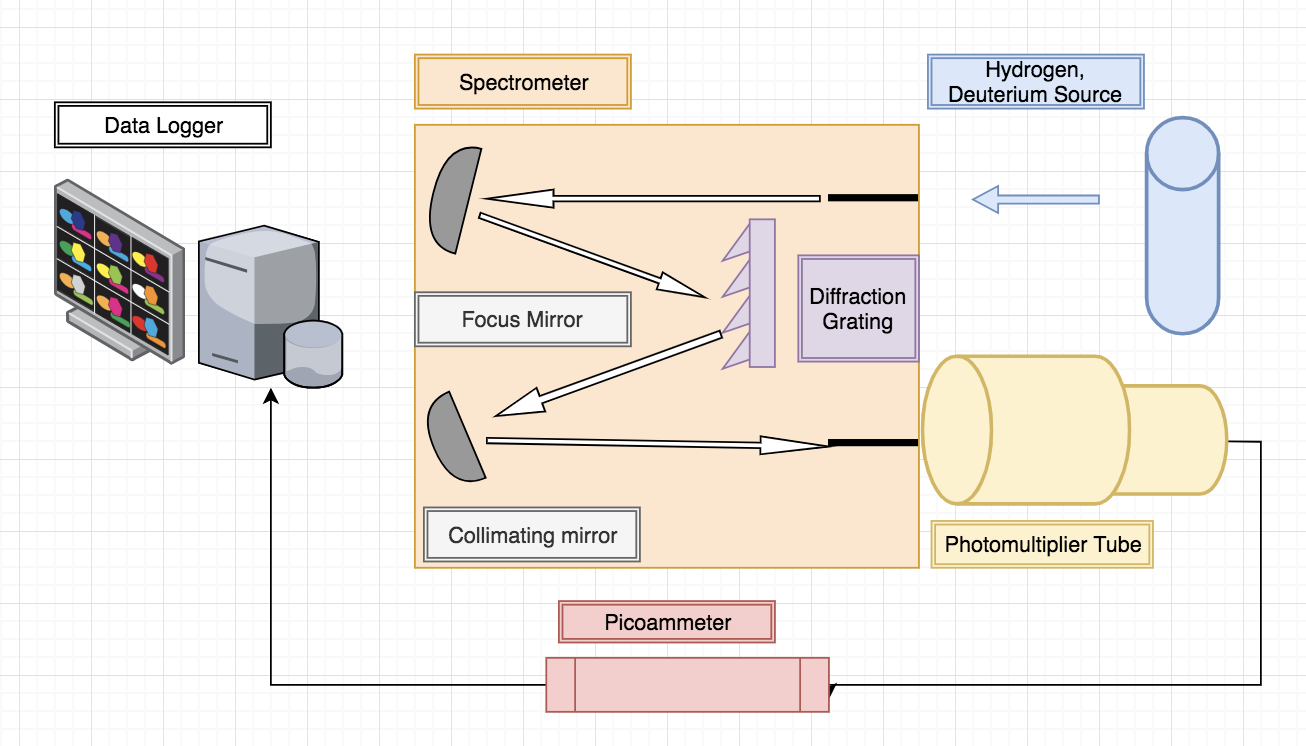
\includegraphics[width=\linewidth]{expDiagram.png}
  \caption{The figure above is a schematic of the experiment design. A $H_2$ and $D_2$ glow discharge emits light into the entry slit of the spectrometer. The spectrometer filters and detects the signal as a current  }
  \label{fig:boat1}
\end{center}
\end{figure}

\begin{figure}[H]
\begin{center}
  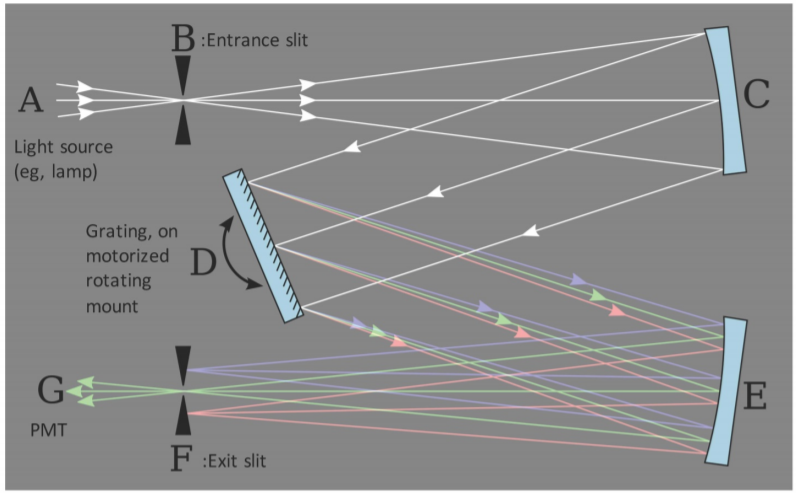
\includegraphics[height = 6cm, width=10cm]{specDiagram.png}
  \caption{The diffraction grating is an optical component that splits and diffracts light into several beams travelling in different directions. The angle at which the grating is at with respect to the vertical determines what wavelength exists the slit. All other wavelengths will not pass through. This is integral in determining the flux as a function of wavelength for a certain source.}
  \label{fig:boat1}
\end{center}
\end{figure}


\section{Results}
We made measurements for the first six Hydrogen and Deuterium Balmer spectral lines. With minor adjustments made to entrance slit and output slits the resolution for each emitted spectral line provided us with distinct peaks allowing us to accurately find the difference in time between the maximum values of each. An example measurement shown in Figure 3 shows the relative peak heights where their different maximum amplitudes can be attributed a increased nucleus mass in Deuterium, which bounds the single electron closer to the nucleus. Peak heights tended toward smaller amplitudes as wavelength decreased, the reason is because these energy transitions are less common than the smaller and produce less photons. This required adjustments to the apparatus in order to take data with low signal to noise ratio.

\begin{figure}[H]
\begin{center}
  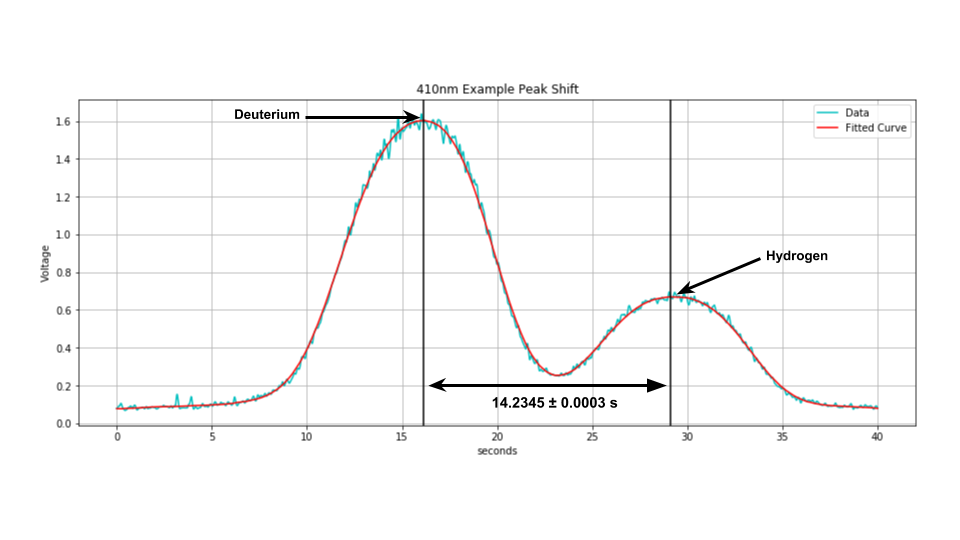
\includegraphics[height = 7cm, width= 13cm]{410_Peak_shift_4.png}
  \caption{The figure above depicts the signal in volts as a function of time with a sweeping speed of $5$ Angstroms per second. The cyan points represent the raw data and the red line represents the transformed filtered data, which gives us a better idea of finding the local maximum of the two gaussian signals.}
  \label{fig:boat1}
\end{center}
\end{figure}


\begin{table}[H]
\centering
\begin{tabular}{ |p{1.8cm}|p{3cm}|p{3.2cm}|p{1.5cm}|}
\hline
Transition & Measured shift(\AA)  & Theoretical shift(\AA ) &  \% Error \\
\hline
$3 \rightarrow 2$ &1.766 \pm 0.019  &1.787 $\AA$ & 1.2\% \\
$4 \rightarrow 2$ &1.301 \pm 0.007
 &1.324& 1.7\% \\
$5 \rightarrow 2$ & 1.186 \pm 0.012 &1.182 & 0.3\% \\
$6 \rightarrow 2$ &1.103 \pm 0.009& $1.059   & 2.9\% \\
$7 \rightarrow 2$ &1.098 \pm 0.004 &1.080  & 1.7\%\\
$8 \rightarrow 2$ &1.062\pm 0.011& $1.059  & 0.3\% \\
\hline
\end{tabular}
\end{table}



\section{Outlook}
In conclusion the isotope shifts for Hydrogen and Deuterium, was successful determined by experiment, to an accurate and precise degree, when compared to theoretical values. Precision in spectroscopy is a challenging feat to overcome, and so statistical methods are necessary when concluding measurements. Potential improvements for future experiment may include an enclosed area, and stronger source signal to decrease signal noise, more calibration measurements, including higher order terms for calibration equation, an increased amount of measurements for HD-shifts, in order to provide a more precise average and lower standard error. 

\end{document}
